\lab{The Discrete Fourier Transform}{The Discrete Fourier Transform}
\objective{The analysis of periodic functions has many applications in pure and applied mathematics, especially in settings dealing with sound waves.
The Fourier transform provides a way to analyze such periodic functions.
In this lab, we introduce how to work with digital audio signals in Python, implement the discrete Fourier transform, and use the Fourier transform to detect the frequencies present in a given sound wave.
We strongly recommend completing the exercises in a Jupyter Notebook.}

\section*{Digital Audio Signals} % ============================================

Sound waves have two important characteristics: \emph{frequency}, which determines the pitch of the sound, and \emph{intensity} or \emph{amplitude}, which determines the volume of the sound.
Computers use \emph{digital audio signals} to approximate sound waves.
These signals have two key components: \emph{sample rate}, which relates to the frequency of sound waves, and \emph{samples}, which measure the amplitude of sound waves at a specific instant in time.

To see why the sample rate is necessary, consider an array with samples from a sound wave.
The sound wave can be arbitrarily stretched or compressed to make a variety of sounds.
If compressed, the sound becomes shorter and has a higher pitch.
Similarly, the same set of samples with a lower sample rate becomes stretched and has a lower pitch.
% This is shown by Figure \ref{fig:DFT_comp_wave}.

\begin{figure}[H]
\captionsetup[subfigure]{justification=centering}
\centering
\begin{subfigure}{.425\textwidth}
    \centering
    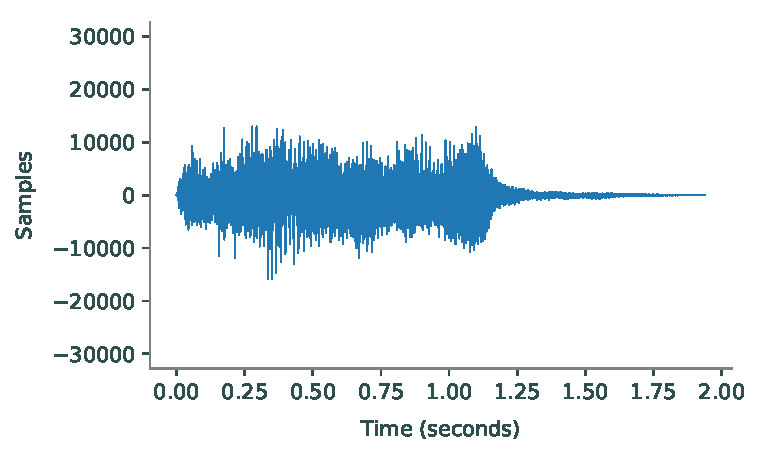
\includegraphics[width=\linewidth]{figures/tada.pdf}
    \caption{The plot of \texttt{tada.wav}.}
    \label{fig:DFT_tada}
\end{subfigure}
\qquad
\begin{subfigure}{.425\textwidth}
    \centering
    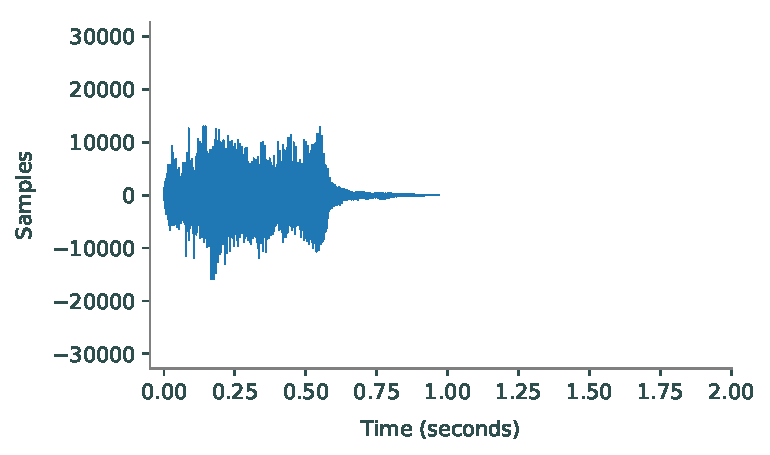
\includegraphics[width=\linewidth]{figures/fast_tada.pdf}
    \caption{Compressed plot of \texttt{tada.wav}.}
    \label{fig:DFT_fasttada}
\end{subfigure}
\caption{Plots of the same set of samples from a sound wave with varying sample rates.
The plot on the left is the plot of the samples with the original sample rate.
The sample rate of the plot on the right has been doubled, resulting in a compression of the actual sound when played back.}
\label{fig:DFT_comp_wave}
\end{figure}

Given the rate at which a set of samples is taken, the wave can be reconstructed exactly as it was recorded.
In most applications, this sample rate is measured in \emph{Hertz} (Hz), the number of samples taken per second.
% \footnote{Hertz is ``cycles per second'' and has units $1/s$.}
The standard rate for high quality audio is $44100$ equally spaced samples per second, or $44.1$ kHz.

\subsection*{Wave File Format} % ----------------------------------------------

One of the most common audio file formats across operating systems is the \emph{wave} format, also called \texttt{wav} after its file extension.
SciPy has built-in tools to read and create \texttt{wav} files.
To read a \texttt{wav} file, use \li{scipy.io.wavfile.read()}.
This function returns the signal's sample rate and its samples.

\begin{lstlisting}
# Read from the sound file.
>>> from scipy.io import wavfile
>>> rate, samples = wavfile.read("tada.wav")
\end{lstlisting}

Sound waves can be visualized by plotting time against the amplitude of the sound, as in Figure \ref{fig:DFT_comp_wave}.
% This plots in the \emph{time domain}.
The amplitude of the sound at a given time is just the value of the sample at that time.
Since the sample rate is given in samples per second, the length of the sound wave in seconds is found by dividing the number of samples by the sample rate:
\begin{align}
\label{eq:dft-xaxis-time}
\frac{\mbox{num samples}}{\mbox{sample rate}}
= \frac{\mbox{num samples}}{\mbox{num samples/second}}
= \mbox{second.}
\end{align}

\begin{problem} % SoundWave.__init__(), SoundWave.plot().
Write a \li{SoundWave} class for storing digital audio signals.
\begin{enumerate}
\item The constructor should accept an integer sample rate and an array of samples.
Store each input as an attribute.
\item Write a method that plots the stored sound wave.
Use \eqref{eq:dft-xaxis-time} to correctly label the $x$-axis in terms of seconds, and set the $y$-axis limits to $[-32768,32767]$ (the reason for this is discussed in the next section).
\end{enumerate}
Use SciPy to read \texttt{tada.wav}, then instantiate a corresponding \li{SoundWave} object and display its plot.
Compare your plot to Figure \ref{fig:DFT_tada}.
\label{prob:fft-SoundWave-init}
\end{problem}

\subsection*{Scaling} % -------------------------------------------------------

To write to a \texttt{wav} file, use \li{scipy.io.wavfile.write()}.
This function accepts the name of the file to write to, the sample rate, and the array of samples as parameters.

\begin{lstlisting}
>>> import numpy as np

# Write a 2-second random sound wave sampled at a rate of 44100 Hz.
>>> samples = np.random.randint(-32768, 32767, 88200, dtype=np.int16)
>>> wavfile.write("white_noise.wav", 44100, samples)
\end{lstlisting}

For \li{scipy.io.wavfile.write()} to correctly create a \texttt{wav} file, the samples must be one of four numerical datatypes: 32-bit floating point (\li{np.float32}), 32-bit integers (\li{np.int32}), 16-bit integers (\li{np.int16}), or 8-bit unsigned integers (\li{np.uint8}).
If samples of a different type are passed into the function, it may still write a file, but the sound will likely be distorted in some way.
In this lab, we only work with 16-bit integer samples, unless otherwise specified.

A 16-bit integer is an integer between $-32768$ and $32767$, inclusive.
If the elements of an array of samples are not all within this range, the samples must be scaled before writing to a file: multiply the samples by 32767 (the largest number in the 16-bit range) and divide by the largest sample magnitude.
This ensures the most accurate representation of the sound and sets it to full volume.
\begin{align}
\label{eq:dft-scale-samples}
\texttt{np.int16}\left(\frac{\mbox{original samples $\times$ 32767}}{\mbox{$\max$(|original samples|)}}\right) = \mbox{scaled samples}
\end{align}

Samples may sometimes contain complex values, especially after some processing.
Make sure to scale and export only the real part (use the \li{real} attribute of the array).

\begin{info} % Embedding sound in a Jupyter Notebook
The IPython API includes a tool for embedding sounds in a Jupyter Notebook.
The function \li{IPython.display.Audio()} accepts either a file name or a sample rate (\li{rate}) and an array of samples (\li{data}); calling the function generates an interactive music player in the Notebook.
\begin{center}
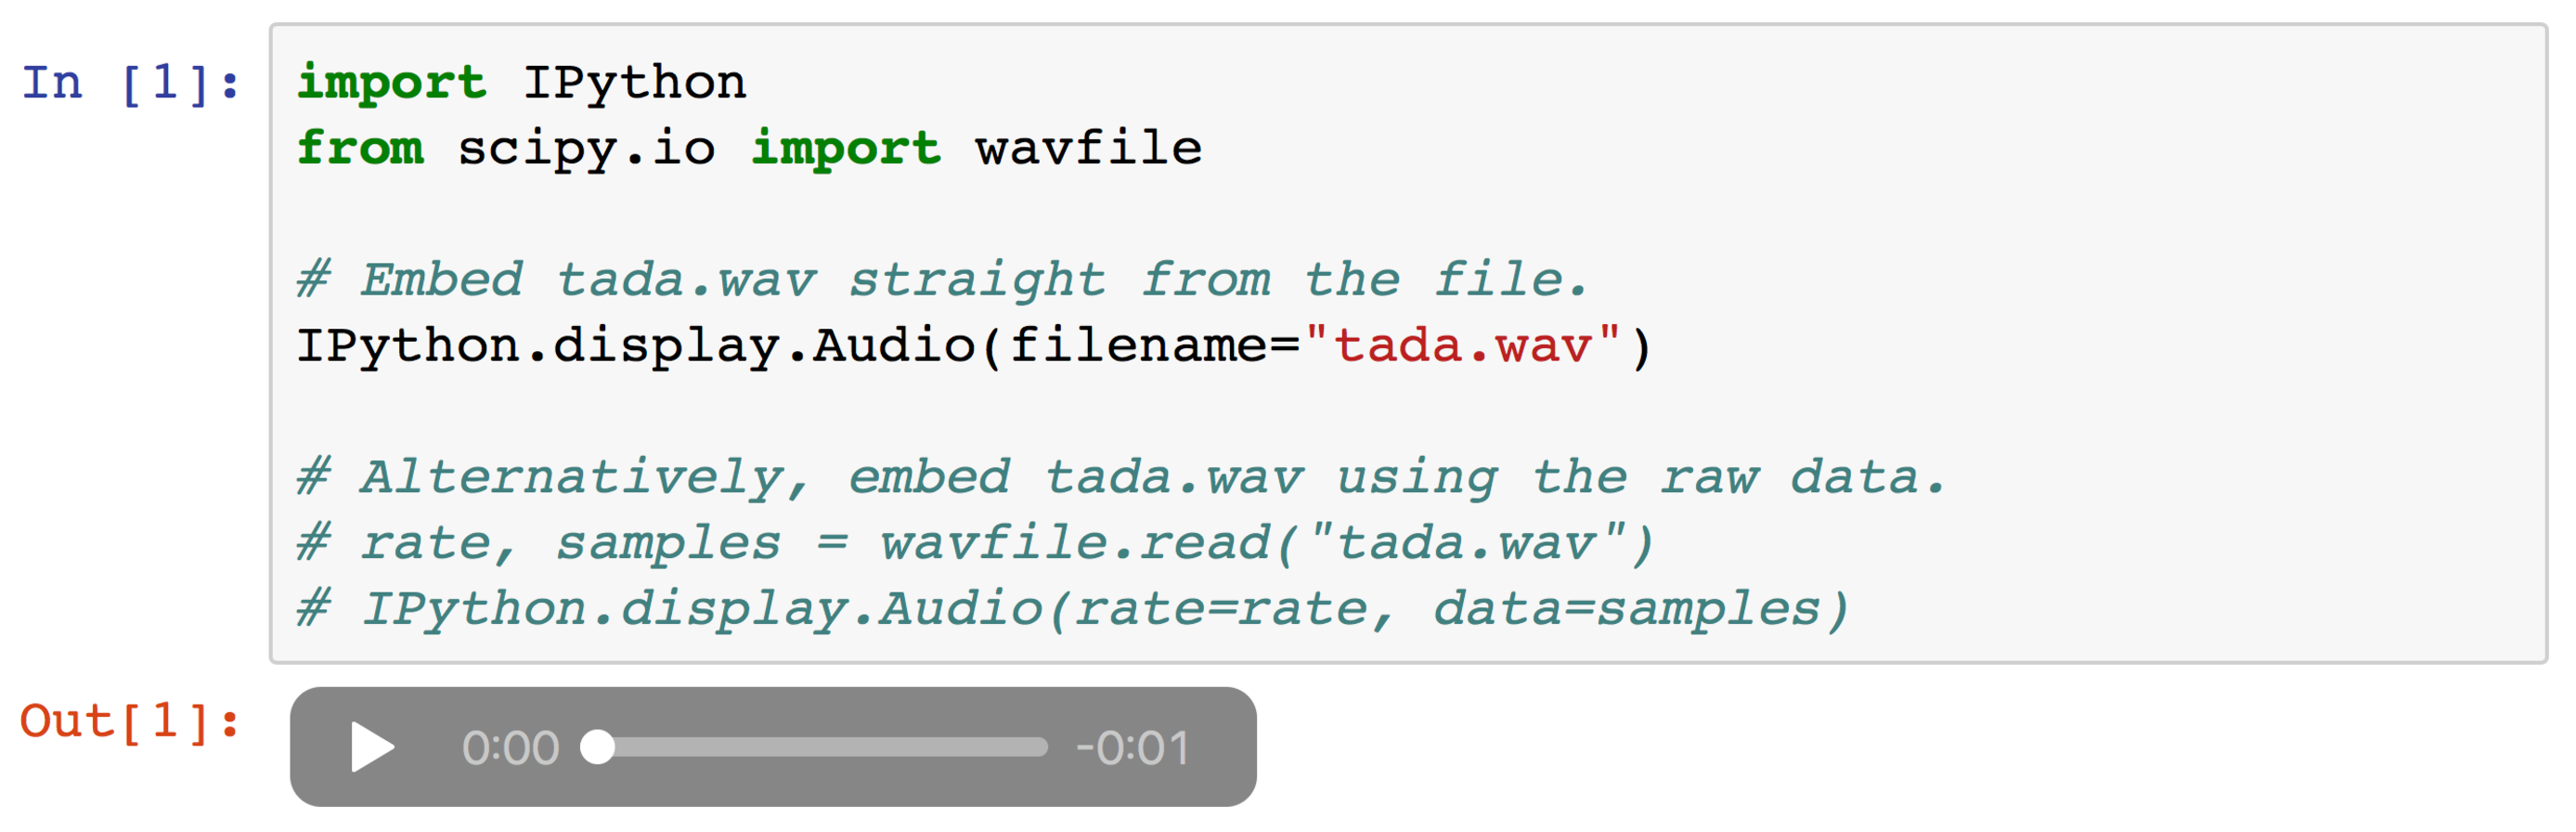
\includegraphics[width=\textwidth]{figures/notebook_audio.pdf}
\end{center}
% See \href{https://ipython.readthedocs.io/en/stable/api/generated/IPython.display.html?highlight=display.Audio}{\texttt{https://ipython.readthedocs.io/en/stable/api/generated/IPython.display.html}} for more info.
\end{info}

\begin{warn}
\textbf{Turn the volume down before listening to any of the sounds in this lab.}
%, especially if you are using headphones.
\end{warn}

\begin{problem} % SoundWave.export().
Add a method to the \li{SoundWave} class that accepts a file name and a boolean \li{force}.
Write to the specified file using the stored sample rate and the array of samples.
If the array of samples does not have \li{np.int16} as its data type, or if \li{force} is \li{True}, scale the samples as in \eqref{eq:dft-scale-samples} before writing the file.

Use your method to create two new files that contains the same sound as \texttt{tada.wav}: one without scaling, and one with scaling (use \li{force=True}).
Use \li{IPython.display.Audio()} to display \texttt{tada.wav} and the new files.
All three files should sound identical, except the scaled file should be louder than the other two.
\end{problem}

\section*{Generating Sounds} % ================================================

Sinusoidal waves correspond to pure frequencies, like a single note on the piano.
Recall that the function $\sin(x)$ has a period of $2\pi$.
To create a specific tone for $1$ second, we sample from the sinusoid with period $1$,
\[
f(x) = \sin(2\pi xk),
\]
where $k$ is the desired frequency.
According to \eqref{eq:dft-xaxis-time}, generating a sound that lasts for $s$ seconds at a sample rate $r$ requires $rs$ equally spaced samples in the interval $[0, s]$. % (these are the $x$ values).

\begin{problem} % Generate simple tones.
Write a function that accepts floats $k$ and $s$.
Create a \li{SoundWave} instance containing a tone with frequency $k$ that lasts for $s$ seconds.
Use a sample rate of $r = 44100$.

The following table shows some frequencies that correspond to common notes.
Octaves of these notes are obtained by doubling or halving these frequencies.
\begin{center}
\begin{tabular}{c|c}
Note & Frequency (Hz) \\
\hline
A & $440$ \\
B & $493.88$ \\
C & $523.25$ \\
D & $587.33$ \\
E & $659.25$ \\
F & $698.46$ \\
G & $783.99$ \\
A & $880$ \\
\end{tabular}
\end{center}
Use your function to generate an A tone lasting for 2 seconds.
\label{prob:generate_note}
\end{problem}

\begin{problem} % Make a chord and a changing sound.
Digital audio signals can be combined by addition or concatenation.
Adding samples overlays tones so they play simultaneously; concatenated samples plays one set of samples after the other with no overlap.

\begin{enumerate}
\item Implement the \li{__add__()} magic method for the \li{SoundWave} class so that if \li{A} and \li{B} are \li{SoundWave} instances, \li{A + B} creates a new \li{SoundWave} object whose samples are the element-wise sum of the samples from \li{A} and \li{B}.
Raise a \li{ValueError} if the sample arrays from \li{A} and \li{B} are not the same length.

Use your method to generate a three-second A minor chord (A, C, and E together).

\item Implement the \li{__rshift__()} magic method\footnote{The \lstinline[basicstyle=\footnotesize\ttfamily]{>>} operator is a \emph{bitwise shift operator} and is usually reserved for operating on binary numbers.} for the \li{SoundWave} class so that if \li{A} and \li{B} are \li{SoundWave} instances, \li{A >> B} creates a new \li{SoundWave} object whose samples are the concatenation of the samples from \li{A}, then the samples from \li{B}.
Raise a \li{ValueError} if the sample rates from the two objects are not equal.
\\(Hint: \li{np.concatenate()}, \li{np.hstack()}, and/or \li{np.append()} may be useful.)

Use your method to generate the arpeggio A $\rightarrow$ C $\rightarrow$ E, where each pitch lasts one second.

\end{enumerate}
Consider using these two methods to produce elementary versions of some simple tunes.
\label{prob:minor_chord_example}
\end{problem}

\section*{The Discrete Fourier Transform} % ===================================

Under the right conditions, a continuous periodic function $f$ with period $T$ (meaning $f(t + T) = f(t)$ for all $t$) may be represented as a weighted sum of exponentials, i.e.,
\begin{align*}
f(x) = \sum_{k=-\infty}^{\infty} c_k e^{2\pi i k x / T}.
\end{align*}
The constants $c_k$ are called the \emph{Fourier coefficients}. % and correspond to the \emph{continuous Fourier transform}.
% The frequencies present in the continuous case are multiples of a sine wave with a period of 1.

The \emph{discrete Fourier transform} (DFT) transforms a discrete array of samples to an array of corresponding Fourier coefficients.
For an array of $n$ samples $\f = \begin{bmatrix}f_0 & f_1 & \cdots & f_{n-1}\end{bmatrix}\trp$, the $k$th coefficient of the DFT of $\f$ is calculated as
\begin{align}
\label{eq:dft-kth-coefficient}
c_k = \frac{1}{n}\sum_{\ell=0}^{n-1} \f_\ell e^{-2\pi i k \ell / n},
\end{align}
where $i = \sqrt{-1}$ is the imaginary unit (\li{1j} in Python).
Repeating this process for each $k$ yields the DFT array of coefficients $\c = \begin{bmatrix}c_0 & c_1 & \cdots & c_{n-1}\end{bmatrix}\trp$.
% Thus, there are as many Fourier coefficients as samples from the original sound wave.
We write $F_n\f = \c$ to indicate that the DFT depends on the number of samples $n$.

\begin{warn}
There are several different conventions for defining the DFT.
For example, instead of \eqref{eq:dft-kth-coefficient}, \li{scipy.fftpack.fft()} uses the formula
\begin{align*}
\hat{c}_k = \sum_{\ell=0}^{n-1} \f_\ell e^{-2\pi i k \ell / n},
\end{align*}
which is \eqref{eq:dft-kth-coefficient} without the factor of $1/n$ in front of the sum.
Denoting this version of the DFT as $\hat{F}_n\f = \hat{\c}$, we have $nF_n = \hat{F}_n$ and $n\c = \hat{\c}$.
The conversion is easy, but it is very important to be aware of which convention a particular implementation of the DFT uses.
\end{warn}

\begin{problem} % naive DFT.
Write a function that accepts an array $\f$ of samples.
Use \eqref{eq:dft-kth-coefficient} to calculate the DFT of $\f$ (including the $1/n$ scaling in front of the sum).

Test your implementation on small, random arrays against \li{scipy.fftpack.fft()}, scaling your output $\c$ to match SciPy's output $\hat{\c}$. % and scipy.fft().
Once your function is working, try to optimize it so that each coefficient $c_k$ is calculated in just one line of code, or---better yet---so that the entire array of coefficients is calculated in the one line.
\\(Hint: use array broadcasting to represent $F_n$ as an $n\times n$ matrix.)
\label{prob:dft-naive}
\end{problem}

\subsection*{The Fast Fourier Transform} % ------------------------------------

Calculating the DFT of a vector of $n$ samples using only (\ref{eq:dft-kth-coefficient}) is at least $O(n^2)$, which is incredibly slow for realistic sound waves.
Fortunately, due to its inherent symmetry, the DFT can be implemented as a recursive algorithm by separating the computation into even and odd indices.
This method of calculating the DFT is called the \emph{fast Fourier transform} (FFT) and runs in $O(n\log{n})$ time.

\begin{algorithm}[H]
\begin{algorithmic}[1]
\Procedure{simple\_fft}{$\f$, $N$}
    \Procedure{split}{$\g$}
        \State $n \gets \size{\g}$
        \If{$n \le N$}
            \label{step:fft-base-case-a}
            \State \pseudoli{return} $n F_n \g$
                \Comment{Use the function from Problem \ref{prob:dft-naive} for small enough $\g$.}
                \label{step:fft-base-case-b}
        \Else{}
            \State \li{even} $\gets$ \li{SPLIT}$(\g_{::2})$
                \Comment{Get the DFT of every other entry of $\g$, starting from $0$.}
            \State \li{odd} $\gets$ \li{SPLIT}$(\g_{1::2})$
                \Comment{Get the DFT of every other entry of $\g$, starting from $1$.}
            \State $\z \gets\zeros{n}$
            \For{$k = 0,1,\ldots,n-1$}
                \Comment{Calculate the exponential parts of the sum.}
                \label{step:fft-loop-a}
                \State $z_k \gets e^{-2\pi i k / n}$
                    % \Comment{This part can be done with array broadcasting.}
                    \label{step:fft-loop-b}
            \EndFor
            \State{$m \gets n\,$\li{//}$\,2$}
                \Comment{Get the middle index for $\z$ (\li{//} is integer division).}
            \State \pseudoli{return} $[$\li{even}$\ +\ \z_{:m} \odot $\li{odd}$,\ $\li{even}$\ +\ \z_{m:} \odot $\li{odd}$]$
                \Comment{Concatenate two arrays of length $m$.}
                % \Comment{$\odot$ is component-wise multiplication.}
                \label{step:fft-concatenate}
        \EndIf
    \EndProcedure
    \State \pseudoli{return} \li{SPLIT}$(\f)\,/\,\size{\f}$
\EndProcedure
\end{algorithmic}
\caption{The fast Fourier transform for arrays with $2^a$ entries for some $a \in \mathbb{N}$.}
\label{alg:FFT}
\end{algorithm}

Note that the base case in lines \ref{step:fft-base-case-a}--\ref{step:fft-base-case-b} of Algorithm \ref{alg:FFT} results from setting $n = 1$ in \eqref{eq:dft-kth-coefficient}, yielding the single coefficient $c_0 = g_0$.
The $\odot$ in line \ref{step:fft-concatenate} indicates the component-wise product
\begin{align*}
\f\odot\g = \begin{bmatrix}f_0g_0 & f_1g_1 & \cdots & f_{n-1}g_{n-1}\end{bmatrix}\trp,
\end{align*}
which is also called the \emph{Hadamard product} of $\f$ and $\g$.

This algorithm performs significantly better than the na\"ive implementation for \eqref{eq:dft-kth-coefficient}, but the simple version described in Algorithm \ref{alg:FFT} only works if the number of original samples is exactly a power of $2$.
SciPy's FFT routines avoid this problem by padding the sample array with zeros until the size is a power of $2$, then executing the remainder of the algorithm from there. % TODO: This might not be true!! See https://stackoverflow.com/questions/6855169/convolution-computations-in-numpy-scipy.
Of course, SciPy also uses various other tricks to further speed up the computation.

\begin{problem} % simple FFT.
Write a function that accepts an array $\f$ of $n$ samples where $n$ is a power of $2$.
Use Algorithm \ref{alg:FFT} to calculate the DFT of $\f$.
\\(Hint: eliminate the loop in lines \ref{step:fft-loop-a}--\ref{step:fft-loop-b} with \li{np.arange()} and array broadcasting, and use \li{np.concatenate()} or \li{np.hstack()} for the concatenation in line \ref{step:fft-concatenate}.)

Test your implementation on random arrays against \li{scipy.fftpack.fft()}, scaling your output $\c$ to match SciPy's output $\hat{\c}$.
Time your function from Problem \ref{prob:dft-naive}, this function, and SciPy's function on an array with $8192$ entries.
\\(Hint: Use \li{<p<\%time>p>} in Jupyter Notebook to time a single line of code.)
\label{prob:fft-simple}
\end{problem}

\section*{Visualizing the DFT} % ==============================================

The graph of the DFT of a sound wave is useful in a variety of applications.
While the graph of the sound in the time domain gives information about the amplitude (volume) of a sound wave at a given time, the graph of the DFT shows which frequencies (pitches) are present in the sound wave.
Plotting a sound's DFT is referred to as plotting in the \emph{frequency domain}.

As a simple example, the single-tone notes generated by the function in Problem \ref{prob:generate_note} contain only one frequency.
For instance, Figure \ref{fig:dft_a} graphs the DFT of an A tone.
However, this plot shows two frequency spikes, despite there being only one frequency present in the actual sound.
This is due to symmetries inherent to the DFT; for frequency detection, the second half of the plot can be ignored as in Figure \ref{fig:dft_a_half}.

\begin{figure}[H]
\captionsetup[subfigure]{justification=centering}
\centering
\begin{subfigure}{.49\textwidth}
    \centering
    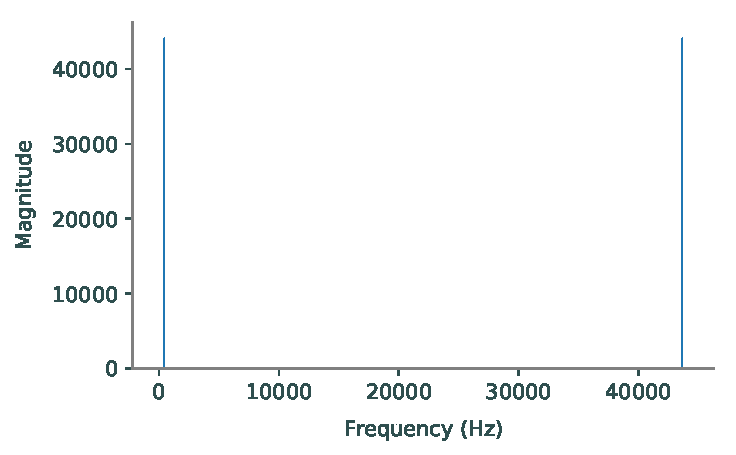
\includegraphics[width=\linewidth]{figures/dft_a.pdf}
    \caption{The DFT of an A tone with symmetries.}
    \label{fig:dft_a}
\end{subfigure}
% \qquad
\begin{subfigure}{.49\textwidth}
    \centering
    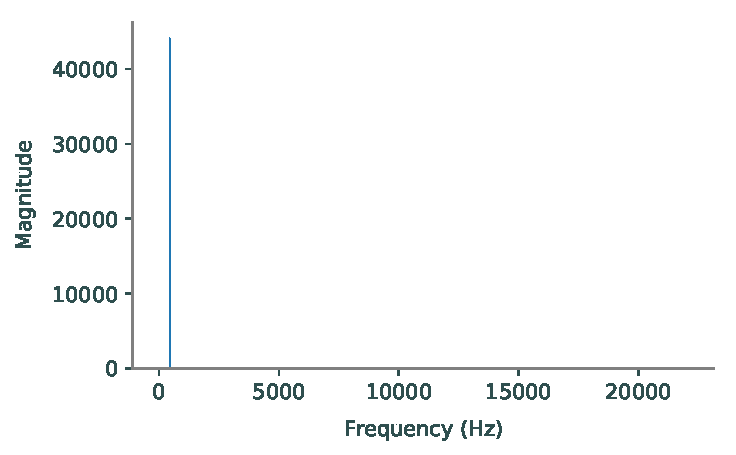
\includegraphics[width=\linewidth]{figures/dft_a_half.pdf}
    \caption{The DFT of an A tone without symmetries.}
    \label{fig:dft_a_half}
\end{subfigure}
\caption{Plots of the DFT with and without symmetries.
Notice that the $x$-axis of the symmetrical plot on the left goes up to $44100$ (the sample rate of the sound wave) while the $x$-axis of the non-symmetric plot on the right goes up to only $22050$ (half the sample rate).
Also notice that the spikes occur at $440$ Hz and $43660$ Hz (which is $44100 - 440$).}
\end{figure}

The DFT of a more complicated sound wave has many frequencies, each of which corresponds to a different tone present in the sound wave.
The magnitude of the coefficients indicates a frequency's influence in the sound wave; a greater magnitude means that the frequency is more influential.
% See Figure \ref{fig:dft_tada} for an example.

\begin{figure}[H]
\centering
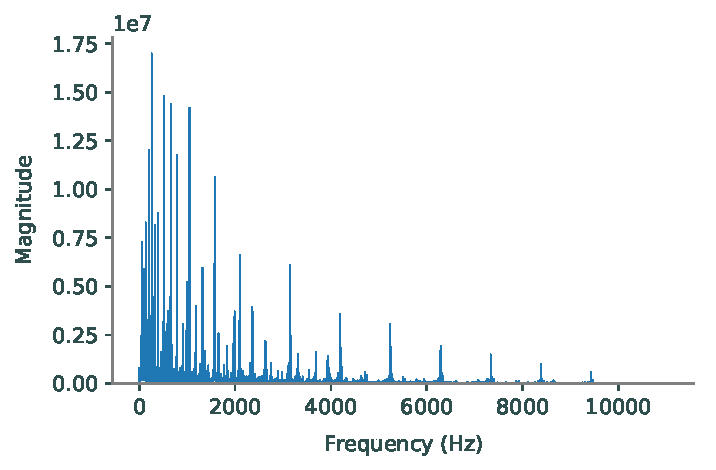
\includegraphics[width=.7\textwidth]{figures/dft_tada.pdf}
\caption{The discrete Fourier transform of \texttt{tada.wav}.
Each spike in the graph corresponds to a frequency present in the sound wave.
Since the sample rate of \texttt{tada.wav} is $22050$ Hz, the plot of its DFT without symmetries only goes up to $11025$ Hz, half of its sample rate.}
\label{fig:dft_tada}
\end{figure}

\subsection*{Plotting Frequencies} % ------------------------------------------

Since the DFT represents the frequency domain, the $x$-axis of a plot of the DFT should be in terms of Hertz, which has units $1/s$.
In other words, to plot the magnitudes of the Fourier coefficients against the correct frequencies, we must convert the frequency index $k$ of each $c_k$ to Hertz.
This can be done by multiplying the index by the sample rate and dividing by the number of samples:
\begin{align}
\label{eq:fft-cycles-conversion}
\frac{k}{\mbox{num samples}} \times \frac{\mbox{num samples}}{\mbox{second}}
= \frac{k}{\mbox{second}}.
% = k\ \mbox{Hz}
\end{align}
In other words, $kr/n = v$, where $r$ is the sample rate, $n$ is the number of samples, and $v$ is the resulting frequency.

% Plotting the DFT of a sound wave without any other considerations results in an $x$-axis that corresponds to the index of the coefficients in the DFT, not their frequencies.
% To label the $x$-axis with the frequencies measured in Hz, or cycles per second, the units must be converted.
% The sample rate is measured in samples per second, so dividing the frequency index by the number of samples and multiplying by the sample rate results in cycles per second, or Hz.

\begin{problem} % plotting the DFT.
Modify your \li{SoundWave} plotting method from Problem \ref{prob:fft-SoundWave-init} so that it accepts a boolean defaulting to \li{False}.
If the boolean is \li{True}, take the DFT of the stored samples and plot---in a new subplot---the frequencies present on the $x$-axis and the magnitudes of those frequencies (use \li{np.<<abs>>()} to compute the magnitude) on the $y$-axis.
Only display the first half of the plot (as in Figures \ref{fig:dft_a_half} and \ref{fig:dft_a_half}), and use \eqref{eq:fft-cycles-conversion} to adjust the $x$-axis so that it correctly shows the frequencies in Hertz.
Use SciPy to calculate the DFT.

Display the DFT plots of the A tone and the A minor chord from Problem \ref{prob:minor_chord_example}.
Compare your results to Figures \ref{fig:dft_a} and \ref{fig:dft_chord}.
\end{problem}

\begin{figure}[H] % DFT of the minor chord.
\centering
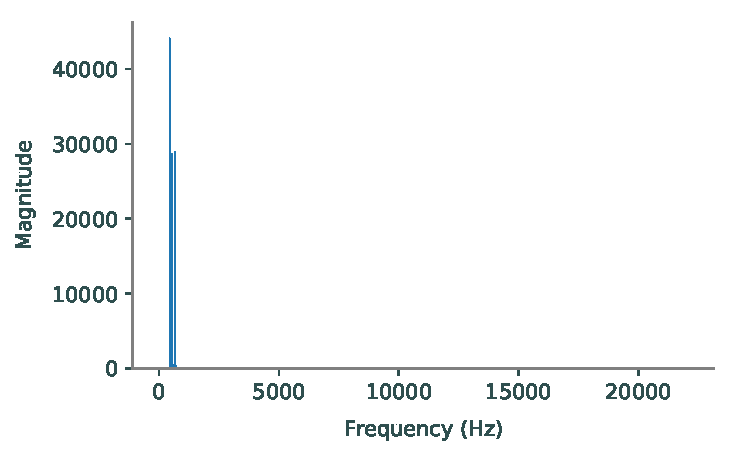
\includegraphics[width=.7\textwidth]{figures/dft_chord.pdf}
\caption{The DFT of the A minor chord.}
\label{fig:dft_chord}
\end{figure}

If the frequencies present in a sound are already known before plotting its DFT, the plot may be interesting, but little new information is actually revealed.
Thus, the main applications of the DFT involve sounds in which the frequencies present are unknown.
One application in particular is sound filtering, which will be explored in greater detail in a subsequent lab.
The first step in filtering a sound is determining the frequencies present in that sound by taking its DFT.

Consider the DFT of the A minor chord in Figure \ref{fig:dft_chord}.
This graph shows that there are three main frequencies present in the sound.
To determine what those frequencies are, find which indices of the array of DFT coefficients have the three largest values, then scale these indices the same way as in \eqref{eq:fft-cycles-conversion} to translate the indices to frequencies in Hertz.

\begin{problem} % Mystery chord.
The file \texttt{mystery\_chord.wav} contains an unknown chord.
Use the DFT and the frequency table in Problem \ref{prob:generate_note} to determine the individual notes that are present in the sound.
\\(Hint: \li{np.argsort()} may be useful.)
\end{problem}

\begin{comment}
\newpage
\section*{Additional Material} % ==============================================

\subsection*{Stereo vs Mono} % ------------------------------------------------

Mono has a single channel so sample arrays are one-dimensional; stereo sounds have channels for left and right speakers, so sample arrays are 2-dimensional: one COLUMN for the left channel, and one COLUMN for the right channel.

\subsection*{Improvements to the SoundWave Class} % ---------------------------

\subsection*{Other Implementations of the FFT} % ------------------------------

FASTEST FOURIER TRANSFORM IN THE WEST!!!
\url{https://en.wikipedia.org/wiki/FFTW}
\url{http://www.fftw.org/}

\end{comment}
